\documentclass[aspectratio=169,10pt]{beamer}

% --- Beamer look & feel ---
\usetheme{Singapore}
\usecolortheme{default}
% \setbeamertemplate{page number in head/foot}[totalframenumber]
\setbeamertemplate{footline}[frame number]
\setbeamertemplate{navigation symbols}{}

\usepackage[T1]{fontenc}
\usepackage[utf8]{inputenc}
\usepackage{lmodern}
\usepackage{tikz}
\usepackage{listings}
\usepackage{xcolor}
\usepackage{booktabs}
\usetikzlibrary{arrows.meta,positioning,shapes.geometric,calc}

\definecolor{codebg}{RGB}{248,248,248}
\definecolor{codeframe}{RGB}{220,220,220}
\definecolor{darkblue}{RGB}{20,60,120}
\definecolor{darkgreen}{RGB}{20,110,70}

\lstdefinelanguage{why3}{
  morekeywords={module,use,export,type,predicate,let,ghost,function,requires,ensures,variant,if,then,else,forall,exists,inductive,lemma,goal,clone,with,val,constant,axiom,match,end,requires,ensures},
  sensitive=true,
  morecomment=[l]{//},
  morecomment=[s]{(*}{*)},
  morestring=[b]"
}

\lstset{
  basicstyle=\ttfamily,
  backgroundcolor=\color{codebg},
  frame=single,
  rulecolor=\color{codeframe},
  breaklines=true,
  columns=fullflexible,
  keepspaces=true,
  showstringspaces=false,
  keywordstyle=\color{darkblue}\bfseries,
  commentstyle=\color{darkgreen},
  tabsize=2
}

\title{Peterson's Algorithm in Why3}
\subtitle{Monolithic Proofs and Refinement for Mutual Exclusion}
\author{Miguel Carvalho (PG61153) \quad\textbullet\quad Margarida Pires (PG61130)}
\date{}

\begin{document}

% 1
\begin{frame}
  \titlepage
  \vspace{-0.6cm}
  \begin{center}
    \small 2-process Peterson's Algorithm \quad $\rightarrow$ \quad N-process Filter algorithm \quad $\rightarrow$ \quad Refinement
  \end{center}
\end{frame}

% 2
\begin{frame}[fragile]{Goal and project structure}
\begin{columns}[T]
\begin{column}{0.43\textwidth}
\textbf{Objective.} Verify mutual exclusion for Peterson-style algorithms in Why3.

\vspace{0.4cm}
\textbf{Main property}
\begin{lstlisting}[language=why3]
forall p q.
  pc[p] = Critical ->
  pc[q] = Critical ->
  p = q
\end{lstlisting}
\end{column}
\begin{column}{0.53\textwidth}
\textbf{Repository}
\begin{lstlisting}
src/
  lib/
    inductiveness.mlw
    refinement.mlw
  monolithic/
    2_processes.mlw
    N_processes.mlw
    N_processes_split_attempt.mlw
  refinement/
    mutual_exclusion_spec.mlw
    filter_abstract.mlw
    filter_concrete_split.mlw
\end{lstlisting}
\end{column}
\end{columns}
\end{frame}

% 3
\begin{frame}[fragile]{Background}
Peterson's algorithm is a mutual exclusion algorithm for shared-memory concurrency.

\vspace{0.3cm}
It does \textbf{not} use a lock or mutex object. Instead, it uses shared variables:

\begin{lstlisting}
turn  : 0..1
want0 : bool
want1 : bool
\end{lstlisting}

\vspace{0.25cm}
The process trying to enter the critical section:
\begin{itemize}
  \item announces interest with \texttt{want};
  \item gives priority to the other process with \texttt{turn};
  \item busy-waits until the guard is true.
\end{itemize}
\end{frame}

% 4
\begin{frame}[fragile]{Two-process Peterson algorithm}

\textbf{Variables}
\begin{lstlisting}[basicstyle=\ttfamily\scriptsize]
var
    turn  : 0..1;
    want0 : boolean = false;
    want1 : boolean = false;
\end{lstlisting}

\vspace{0.3em}

\begin{columns}[T,onlytextwidth]

\begin{column}{0.48\textwidth}
\textbf{\texttt{process0}}
\begin{lstlisting}[basicstyle=\ttfamily\scriptsize]
procedure process0;
begin
    while true do begin
0:      (* idle *)
1:      want0 := true;
2:      turn  := 1;
3:      repeat until (not want1 or turn = 0);
4:      (* critical region *)
5:      want0 := false;
    end
end;
\end{lstlisting}
\end{column}

\begin{column}{0.48\textwidth}
\textbf{\texttt{process1}}
\begin{lstlisting}[basicstyle=\ttfamily\scriptsize]
procedure process1;
begin
    while true do begin
0:      (* idle *)
1:      want1 := true;
2:      turn  := 0;
3:      repeat until (not want0 or turn = 1);
4:      (* critical region *)
5:      want1 := false;
    end
end;
\end{lstlisting}
\end{column}

\end{columns}

\end{frame}

% 5
\begin{frame}[fragile]{2-process Why3 model}
\begin{columns}[T]
\begin{column}{0.48\textwidth}
\textbf{Control states}
\begin{lstlisting}[language=why3]
type process = P0 | P1

type state =
  Zero | One | Two |
  Three | Four | Five
\end{lstlisting}

\textbf{Shared variables}
\begin{lstlisting}[language=why3]
type world = {
  pc   : map process state;
  want : map process bool;
  turn : process;
}
\end{lstlisting}
\end{column}
\begin{column}{0.48\textwidth}
\textbf{Label meaning}
\begin{tabular}{ll}
\toprule
Zero & idle \\
One & set \texttt{want[p]} \\
Two & set \texttt{turn} \\
Three & wait guard \\
Four & critical section \\
Five & reset \texttt{want[p]} \\
\bottomrule
\end{tabular}

\vspace{0.35cm}
\textbf{Result}
\begin{lstlisting}[language=why3]
goal correctness:
  forall w. reachable w ->
    atMostOneCS w
\end{lstlisting}
\end{column}
\end{columns}
\end{frame}

% 6
\begin{frame}[fragile]{2-process invariant idea}
\vspace{0.3cm}
The property \texttt{atMostOneCS} is true, but it is not strong enough by itself.

\vspace{0.3cm}
The inductive invariant records two facts:
\begin{enumerate}
  \item when a process is trying or inside the critical section, \texttt{want[p]} is true;
\begin{lstlisting}[language=why3]
forall p:process.
  interested w p -> w.want[p]
\end{lstlisting}
  \item the waiting process cannot enter while the other is already in the critical section.
\begin{lstlisting}[language=why3]
forall p:process.
  w.pc[p] = Three /\ w.pc[other p] = Four ->
  w.turn = other p
\end{lstlisting}
\end{enumerate}

\vspace{0.1cm}
This gives the standard proof shape:
\[
  reachable(w) \Rightarrow inv(w) \Rightarrow atMostOneCS(w)
\]
\end{frame}

% 7
\begin{frame}[fragile]{From 2 processes to N: Filter algorithm}
\vspace{0.2cm}
For N processes, Peterson's direct two-process structure is replaced by levels.
\vspace{0.1cm}

\begin{lstlisting}[basicstyle=\ttfamily\footnotesize]
var
    level  : array [0..N-1] of integer = [0, ..., 0];
    victim : array [1..N-1] of integer;

procedure process(i);
begin
    while true do begin
0:      (* idle *)
        for l = 1 to N-1 do begin
1:          level[i] := l;
2:          victim[l] := i;
3:          repeat until
              forall k. k != i ->
                level[k] < l or victim[l] != i;
        end;
4:      (* critical region *)
5:      level[i] := 0;
    end
end;
\end{lstlisting}
\end{frame}

% 8
\begin{frame}[fragile]{N-process model in Why3}
\begin{columns}[T]
\begin{column}{0.52\textwidth}
\textbf{Processes and levels}
\begin{lstlisting}[language=why3]
type process = int
type level = int

predicate valid_process p =
  0 <= p < n_processes

predicate valid_level l =
  1 <= l < n_processes
\end{lstlisting}
\end{column}
\begin{column}{0.44\textwidth}
\textbf{Filter variables}
\begin{lstlisting}[language=why3]
type world = {
  pc     : map process state;
  lvl    : map process level;
  victim : map level process;
}
\end{lstlisting}
\end{column}
\end{columns}

\vspace{0.25cm}
\textbf{Waiting guard}
\begin{lstlisting}[language=why3]
predicate waiting_guard (w:world) (p:process) =
  forall q:process.
    valid_process q -> q <> p ->
    w.lvl[q] < w.lvl[p] \/ w.victim[w.lvl[p]] <> p
\end{lstlisting}
\end{frame}

% 9
\begin{frame}[fragile]{Counting invariant for the Filter algorithm}
The key N-process invariant is global and level-indexed.

\begin{lstlisting}[language=why3]
predicate filter_bound (w:world) =
  forall l:level.
    valid_level l ->
    count_passed_level w l n_processes <= n_processes - l
\end{lstlisting}

\vspace{0.2cm}
Interpretation:
\begin{center}
\large At level $l$, at most $N-l$ processes can have passed that level.
\end{center}

\vspace{0.2cm}
At the final level:
\[
  l = N-1 \quad \Rightarrow \quad N-l = 1
\]

Therefore, at most one process can pass the final level, so at most one process can be in the critical section.
\end{frame}

% 10
\begin{frame}{Proof-friendly N-process abstraction}

The proved monolithic N-process model uses an atomic level-entry abstraction.

\vspace{0.2cm}
\begin{center}
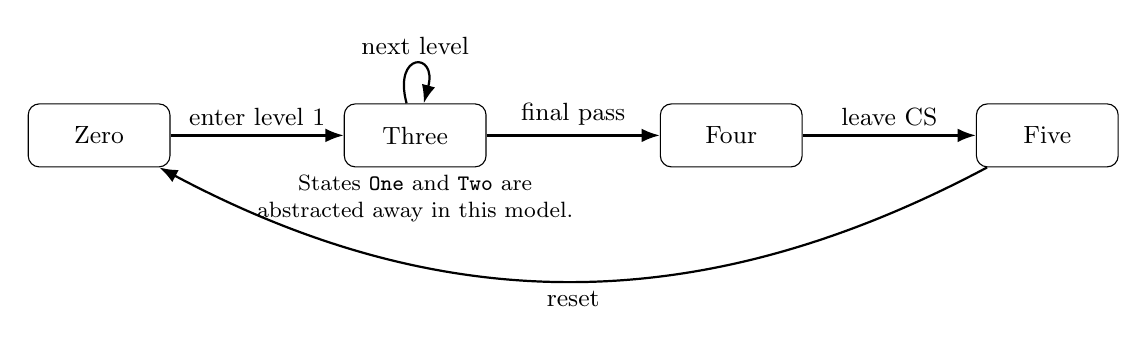
\begin{tikzpicture}[
  node distance=2.2cm,
  every node/.style={font=\small},
  state/.style={draw, rounded corners, minimum width=1.8cm, minimum height=0.8cm},
  >=Latex
]
  \node[state] (z) {Zero};
  \node[state, right=of z] (t) {Three};
  \node[state, right=of t] (f) {Four};
  \node[state, right=of f] (fi) {Five};

  \draw[->, thick] (z) -- node[above]{enter level 1} (t);
  \draw[->, thick] (t) edge[loop above, looseness=8] node[above]{next level} (t);
  \draw[->, thick] (t) -- node[above]{final pass} (f);
  \draw[->, thick] (f) -- node[above]{leave CS} (fi);
  \draw[->, thick] (fi) to[bend left=28] node[below]{reset} (z);

  % clarification note
  \node[align=center, font=\footnotesize] at ($(t)+(0,-0.8)$)
    {States \texttt{One} and \texttt{Two} are\\abstracted away in this model.};
\end{tikzpicture}
\end{center}

\vspace{0.2cm}
This combines:
\begin{center}
\texttt{level[p] := l;} \qquad and \qquad \texttt{victim[l] := p;}
\end{center}

into one proof-friendly transition.
\end{frame}

% 11
\begin{frame}[fragile]{Monolithic proof results}
\begin{block}{Two-process Peterson}
\begin{lstlisting}[language=why3]
goal correctness:
  forall w:world.
    reachable w -> atMostOneCS w
\end{lstlisting}
\end{block}

\begin{block}{N-process abstract Filter model}
\begin{lstlisting}[language=why3]
goal correctness:
  forall w:world.
    reachable w -> atMostOneCS w
\end{lstlisting}
\end{block}

\vspace{0.25cm}
The N-process proof relies on the counting invariant \texttt{filter\_bound} and a lemma showing that two processes counted at the final level must be equal.
\end{frame}

% 12
\begin{frame}{Refinement hierarchy}
\begin{center}
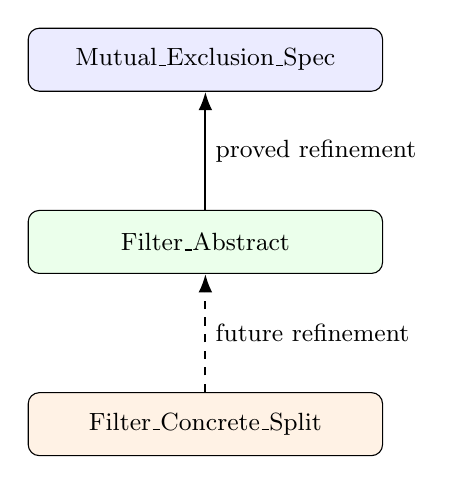
\begin{tikzpicture}[node distance=1.5cm, every node/.style={font=\small}, >=Latex]
  \node[draw, rounded corners, fill=blue!8, minimum width=4.5cm, minimum height=0.8cm] (spec) {Mutual\_Exclusion\_Spec};
  \node[draw, rounded corners, fill=green!8, minimum width=4.5cm, minimum height=0.8cm, below=of spec] (abs) {Filter\_Abstract};
  \node[draw, rounded corners, fill=orange!10, minimum width=4.5cm, minimum height=0.8cm, below=of abs] (conc) {Filter\_Concrete\_Split};
  \draw[->, thick] (abs) -- node[right]{proved refinement} (spec);
  \draw[->, dashed, thick] (conc) -- node[right]{future refinement} (abs);
\end{tikzpicture}
\end{center}
\end{frame}

% 13
\begin{frame}[fragile]{Most abstract model: mutual exclusion spec}
The top-level specification tracks only the control state:

\begin{lstlisting}[language=why3]
type state = Idle | Trying | CS | Exit

type world = {
  pc : map process state;
}
\end{lstlisting}

\vspace{0.2cm}
It does not mention Peterson variables, levels, victims, etc.

\vspace{0.2cm}
The invariant is just the desired safety property:
\begin{lstlisting}[language=why3]
predicate inv (w:world) =
  atMostOneCS w
\end{lstlisting}

\vspace{0.2cm}
A process may enter \texttt{CS} only when no other process is already in \texttt{CS}.
\end{frame}

% 14
\begin{frame}[fragile]{Filter abstraction refines the spec}
The Filter abstraction introduces implementation variables:

\begin{lstlisting}[language=why3]
type world = {
  fpc     : map process Mutual_Exclusion_Spec.state;
  flvl    : map process level;
  fvictim : map level process;
}
\end{lstlisting}

\vspace{0.2cm}
The refinement map hides \texttt{lvl} and \texttt{victim}:

\begin{lstlisting}[language=why3]
let ghost function refn (w:world)
  : Mutual_Exclusion_Spec.world =
  { pc = w.fpc }
\end{lstlisting}

\vspace{0.2cm}
So the abstract specification sees only whether a process is idle, trying, in the critical section, or exiting.
\end{frame}

% 15
\begin{frame}[fragile]{Concrete split-step model and future work}
The concrete split-step model is defined as the next refinement target:

\begin{center}
\small
\texttt{IdleC -> SetLevel -> SetVictim -> TryingC -> CSC -> ExitC -> IdleC}
\end{center}

\vspace{0.2cm}
It separates the doorway instructions:
\begin{lstlisting}
level[i]  := l
victim[l] := i
\end{lstlisting}

\vspace{0.2cm}
Open proof obligation:
\begin{itemize}
  \item define a refinement map hiding \texttt{SetLevel} and \texttt{SetVictim};
  \item abstract partially updated \texttt{lvl} and \texttt{victim};
  \item prove the counting invariant remains inductive for the fully split model.
\end{itemize}
\end{frame}

% 16
\begin{frame}{Conclusion}
\begin{itemize}
  \item Proved mutual exclusion for the original 2-process Peterson algorithm.
  \item Generalized to the N-process Filter algorithm using a proof-friendly abstraction.
  \item Used the standard counting invariant: at level $l$, at most $N-l$ processes can pass.
  \item Built a refinement hierarchy:
  \begin{center}
    \texttt{Filter\_Abstract} refines \texttt{Mutual\_Exclusion\_Spec}
  \end{center}
  \item Included the concrete split-step Filter model as the next refinement target.
  \item Related work: \textcolor{blue}{\href{https://jamesrwilcox.com/SharedMem.html}{A Proof of Peterson's Algorithm (in Coq) by James Wilcox}}.
\end{itemize}

\vspace{0.25cm}
\begin{center}
\large Final result: Why3 proves mutual exclusion for the completed models.
\end{center}
\end{frame}

\end{document}
